%!TEX TS-program = pdflatex
%!TEX encoding = UTF-8 Unicode
%!TEX root = ../2018-03-26-papa-vitres-de-son.tex

%*******************************************************
% Titlepage
%*******************************************************

\begin{titlepage}
\pdfbookmark{Titlepage}{Titlepage}
\changetext{}{}{}{((\paperwidth  - \textwidth) / 2) - \oddsidemargin - \hoffset - 1in}{}
    \begin{center}

\begin{table}[htp]
\begin{center}
\begin{tabular}{rl}
\multirow{ 2}{*}{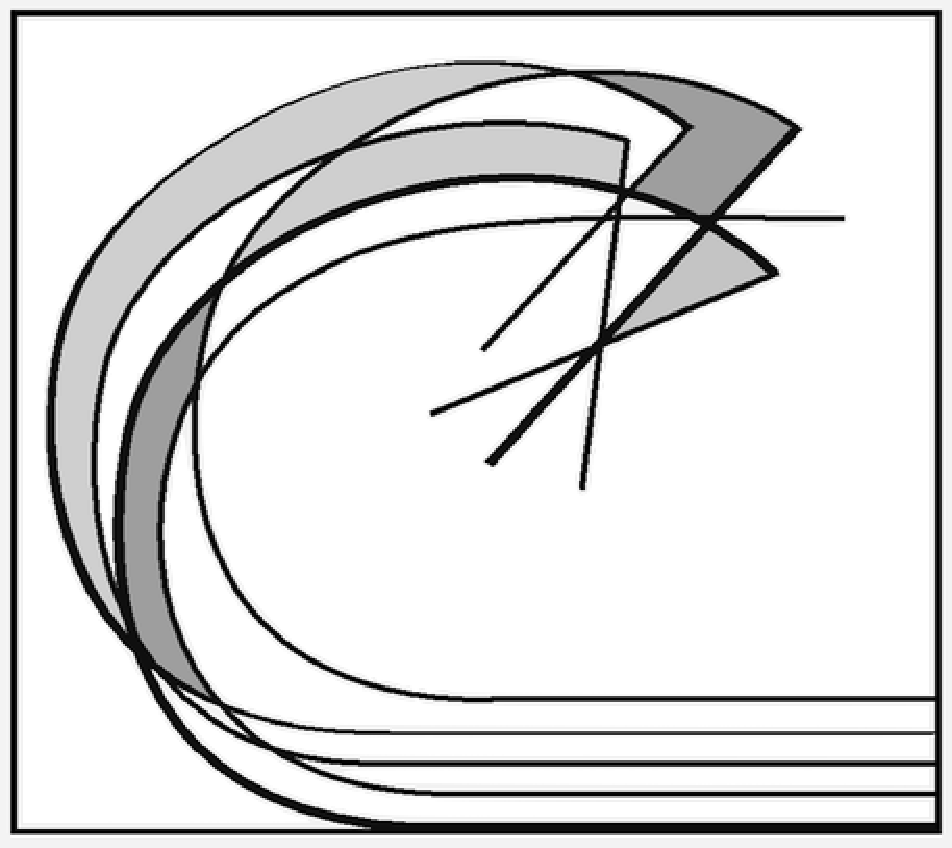
\includegraphics[scale=0.105]{Conservatorio.pdf}} & \LARGE \spacedlowsmallcaps{Conservatorio di Musica S. Cecilia di Roma} \\ \cline{2-2}
& \spacedlowsmallcaps{DIPARTIMENTO DI NUOVE TECNOLOGIE E LINGUAGGI MUSICALI} \\
& \spacedlowsmallcaps{SCUOLA DI MUSICA ELETTRONICA} \\
\end{tabular}
\end{center}
\label{default}
\end{table}%
        
%        \LARGE \spacedlowsmallcaps{Conservatorio di Musica S. Cecilia di Roma}
%        
%        \bigskip
%        
%        \hrule
%        
%        \bigskip
%        
%        \large \spacedlowsmallcaps{DIPARTIMENTO DI NUOVE TECNOLOGIE E LINGUAGGI MUSICALI}
%        
%        \spacedlowsmallcaps{SCUOLA DI MUSICA ELETTRONICA}
        
		\vfill
        
        \spacedlowsmallcaps{CORSO DI DIPLOMA ACCADEMICO DI PRIMO LIVELLO IN}
                       
        \LARGE \spacedlowsmallcaps{MUSICA ELETTRONICA}

        \vfill ~ \vfill

        \LARGE {\color{Maroon}\spacedallcaps{\myTitle}}
        
        \large \mySubTitle 
        
        \vfill
        
        \normalsize Candidato: \\
        \Large \spacedlowsmallcaps{\myName}
        
        \normalsize Matricola: \\
        \Large \spacedlowsmallcaps{2945TR}
        
        \bigskip
        
        \normalsize Relatore: \\
        \Large \spacedlowsmallcaps{Michelangelo Lupone}

        \vfill ~ \vfill ~ \vfill
        
        \normalsize Anno Accademico: \\
        \Large \spacedlowsmallcaps{2016-2017}


%        
\includegraphics[width=0.7\textwidth]{TFZSuperEllisse} \\ \bigskip
                   

    \end{center}        

\end{titlepage} 